% Created 2020-09-11 Fri 01:54
% Intended LaTeX compiler: lualatex
\documentclass[11pt]{article}
\usepackage{graphicx}
\usepackage{grffile}
\usepackage{longtable}
\usepackage{wrapfig}
\usepackage{rotating}
\usepackage[normalem]{ulem}
\usepackage{amsmath}
\usepackage{textcomp}
\usepackage{amssymb}
\usepackage{capt-of}
\usepackage{hyperref}
\usepackage{tabularx}
\usepackage{etoolbox}
\makeatletter
\def\dontdofcolorbox{\renewcommand\fcolorbox[4][]{##4}}
\AtBeginEnvironment{minted}{\dontdofcolorbox}
\makeatother
\usepackage[newfloat]{minted}
\usepackage{amsthm}
\theoremstyle{definition}
\newtheorem{definition}{Definition}[section]
\usepackage{unicode-math}
\usepackage{unicode}
\author{Mark Armstrong}
\date{Fall 2020}
\title{Introduction and overview\\\medskip
\large Principles of Programming Languages}
\hypersetup{
   pdfauthor={Mark Armstrong},
   pdftitle={Introduction and overview},
   pdfkeywords={},
   pdfsubject={An introduction and a brief overview of topics we will discuss in the course.},
   pdfcreator={Emacs 27.0.90 (Org mode 9.3.7)},
   pdflang={English},
   colorlinks,
   linkcolor=blue,
   citecolor=blue,
   urlcolor=blue
   }
\begin{document}

\maketitle

\section{Preamble}
\label{sec:org1e3910e}
The preamble section of each notes will include
\begin{itemize}
\item an introduction to the material covered in the section,
\item any notable references,
\begin{itemize}
\item i.e., specific chapters of our recommended/additional texts
from which the notes are derived, or which expand on the notes,
\end{itemize}
\item a table of contents, and
\item if necessary, an update history, chronicling any major changes.
\begin{itemize}
\item Note the git commit history will provide a more fine-grained
record of upates.
\end{itemize}
\end{itemize}

\subsection{Introduction}
\label{sec:orgb40a370}
This section of notes introduces the course and the staff,
and lays out a few central concepts.

\subsection{Notable references}
\label{sec:orgb5a7431}
\begin{itemize}
\item Peter Van Roy and Seif Haridi,
“\href{http://citeseerx.ist.psu.edu/viewdoc/download?doi=10.1.1.102.7366\&rep=rep1\&type=pdf}{Concepts, Techniques, and Models of Computer Programming}”,
Preface
\item Peter Van Roy, “\href{https://www.info.ucl.ac.be/\~pvr/VanRoyChapter.pdf}{Programming Paradigms for Dummies: What Every Programmer Should Know}”
\item Robert W. Sebesta, “Concepts of Programming Languages” (10th edition)
\end{itemize}

\subsection{Table of comments}
\label{sec:org3b4fd83}

\begin{scriptsize}
\begin{itemize}
\item \hyperref[sec:org1e3910e]{Preamble}
\begin{itemize}
\item \hyperref[sec:orgb40a370]{Introduction}
\item \hyperref[sec:orgb5a7431]{Notable references}
\item \hyperref[sec:org3b4fd83]{Table of comments}
\end{itemize}
\item \hyperref[sec:org42b4ceb]{Welcome}
\begin{itemize}
\item \hyperref[sec:orgfd0aeed]{Instructor: Mark Armstrong}
\item \hyperref[sec:orgee9af86]{Teaching assistant: Habib Ghaffari-Hadigheh}
\end{itemize}
\item \hyperref[sec:orgbb231f4]{Purpose and goals of this course}
\begin{itemize}
\item \hyperref[sec:org4ca375d]{Calendar description}
\item \hyperref[sec:org1af5ad8]{Informal objectives}
\item \hyperref[sec:org6fd6a6f]{Course preconditions}
\item \hyperref[sec:org2a35ad4]{Course postconditions}
\item \hyperref[sec:orgd950a1b]{Formal rubric for the course}
\end{itemize}
\item \hyperref[sec:org86b4671]{“Principles of programming languages”}
\begin{itemize}
\item \hyperref[sec:org5a26242]{What is a programming language?}
\begin{itemize}
\item \hyperref[sec:orgcaf9edf]{Example of a process}
\end{itemize}
\item \hyperref[sec:orgc8d6318]{What are the components of a programming language?}
\begin{itemize}
\item \hyperref[sec:orge1e9532]{Syntax and semantics example}
\item \hyperref[sec:org0adb9e7]{Exercise: a meaningless C or Java program}
\end{itemize}
\item \hyperref[sec:orge8c69ff]{How do we classify a programming language?}
\end{itemize}
\item \hyperref[sec:orgdec9f17]{Abstraction}
\begin{itemize}
\item \hyperref[sec:org1e3910e]{Preamble}
\item \hyperref[sec:org5700042]{Dijkstra on abstraction}
\item \hyperref[sec:orgdbf00c9]{Example: sorting}
\item \hyperref[sec:org88cacb3]{“Leaky” abstractions}
\item \hyperref[sec:org2fd130b]{A taxonomy of programming paradigms by abstraction support}
\item \hyperref[sec:org5445a47]{Abstractions throughout this course}
\end{itemize}
\item \hyperref[sec:org6e1a57f]{Exercises}
\end{itemize}
\end{scriptsize}

\section{Welcome}
\label{sec:org42b4ceb}
\begin{center}
Welcome to the course!
\end{center}

\subsection{Instructor: Mark Armstrong}
\label{sec:orgfd0aeed}
\begin{quote}
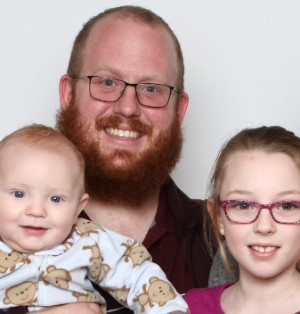
\includegraphics[width=200px]{./media/markarmstrong.jpg}
\end{quote}

\begin{itemize}
\item Email: \href{mailto:armstmp@mcmaster.ca}{armstmp@mcmaster.ca}
\item Website: \url{https://armkeh.github.io}
\end{itemize}

(Digital) office/student conference hours available on request.

\subsection{Teaching assistant: Habib Ghaffari-Hadigheh}
\label{sec:orgee9af86}
\begin{quote}
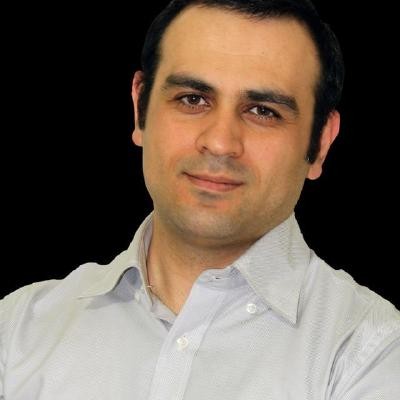
\includegraphics[width=200px]{./media/habibghaffarihadigheh.jpg}
\end{quote}

\begin{itemize}
\item Email: \href{mailto:ghaff1@mcmaster.ca}{ghaffh1@mcmaster.ca}
\item Website: \url{https://ghhabib.me/}
\end{itemize}

(Digital) office/student conference hours available on request.

\section{Purpose and goals of this course}
\label{sec:orgbb231f4}
Here we provide both formal and informal descriptions
and goals for this course.

\subsection{Calendar description}
\label{sec:org4ca375d}
Design space of programming languages;
abstraction and modularization concepts and mechanisms;
programming in non-procedural (functional and logic) paradigms;
introduction to programming language semantics.

\subsection{Informal objectives}
\label{sec:org1af5ad8}
\begin{itemize}
\item Investigate a number of programming languages
which exemplify different paradigms.
\begin{itemize}
\item A relatively shallow but comprehensive survey.
\item Focusing on general-purpose languages.
\end{itemize}
\item \emph{Formally} describe programming language syntax and semantics.
\begin{itemize}
\item An application of theory learned previously.
\end{itemize}
\item Apply various abstraction and modularisation techniques,
\begin{itemize}
\item Learning how to apply them and
to which situations they are best applied.
\end{itemize}
\end{itemize}

\subsection{Course preconditions}
\label{sec:org6fd6a6f}
Before beginning this course:

\begin{enumerate}
\item Students should know and understand:
\begin{enumerate}
\item Basic concepts about integers, sets, functions, \& relations.
\item Induction and recursion.
\item First order logic, axiomatic theories \& simple proof techniques.
\item Regular expressions \& context-free grammars.
\item Programming in imperative languages.
\item Basic concepts of functional programming languages.
\end{enumerate}
\item Students should be able to:
\begin{enumerate}
\item Produce proofs involving quantifiers and/or induction.
\item Understand the meaning of a given axiomatic theory.
\item Construct regular sets \& context-free languages.
\item Produce small to medium scale programs in imperative languages.
\item Produce small scale programs in functional languages.
\end{enumerate}
\end{enumerate}

\subsection{Course postconditions}
\label{sec:org2a35ad4}
After completion of this course:

\begin{enumerate}
\item Students should know and understand:
\begin{enumerate}
\item Programming in functional languages.
\item Programming in logical languages.
\item Formal definitions of syntax \& semantics for various
simple programming languages.
\item Various abstraction \& modularisation techniques
employed in programming languages.
\end{enumerate}
\item Students should be able to:
\begin{enumerate}
\item Reason about the design space of programming languages,
in particular tradeoffs \& design issues.
\item Produce formal descriptions of syntax \& semantics
from informal descriptions, identifying ambiguities.
\item Select appropriate abstraction \& modularisation techniques
for a given problem.
\item Produce tools for domain-specific languages
in imperative, functional and logical languages.
\end{enumerate}
\end{enumerate}

\subsection{Formal rubric for the course}
\label{sec:orgd950a1b}
\begin{scriptsize}
\begin{center}
\begin{tabular}{|l|l|l|l|l|}
\hline
Topic & Below & Marginal & Meets & Exceeds \\
\hline
Familiarity & Shows some & Shows & Achieves & Achieves \\
with various & competence & competence & competence & competence \\
programming & in & in & with the & with \\
languages & procedural & procedural & basic & intermediate \\
 & languages, & languages & usage of & usage of \\
 & but not & and limited & various & various \\
 & languages & competence & languages & languages \\
 & from other & in & & \\
 & paradigms & languages & & \\
 & & from other & & \\
 & & paradigms & & \\
\hline
Ability to & Cannot & Identifies & Identifies & Identifies \\
identify and & consistently & such & such & sucj \\
make use of & identify & constructs, & constructs & constructs \\
abstraction, & such & but does not & and shows & and shows \\
modularisation & constructs & consistently & some ability & mastery of \\
constructs & & make use of & to make use & them when \\
 & & them when & of them when & programming \\
 & & programming & programming & \\
\hline
Ability to & Unable or & Comprehends & Makes only & Consistently \\
comprehend and & rarely & given & minor & fully \\
produce formal & able to & grammars, & errors & understands \\
descriptions & comprehend & but & regarding & given \\
of PL syntax & given & produces & precedence & grammars and \\
 & grammars; & grammars & or & produces \\
 & does not & which are & ambiguity & correct \\
 & identify & ambiguous & when & grammars. \\
 & ambiguity & or which do & reading or & \\
 & or & not & producing & \\
 & precedence & correctly & grammars & \\
 & rules & specify & & \\
 & & precedence & & \\
\hline
Ability to & Rarely or & Usually & Comprehends & Comprehends \\
comprehend and & never & comprehends & such & such \\
produce & comprehends & such semantic & semantic & semantic \\
operational & such & descriptions, & descriptions & descriptions \\
semantics for & semantic & but cannot & and produces & and produces \\
simple PLs & descriptions & consistently & them with & them without \\
 & & produce them & only minor & errors \\
 & & & errors & \\
\hline
\end{tabular}
\end{center}
\end{scriptsize}

\section{“Principles of programming languages”}
\label{sec:org86b4671}
We begin the course with these fundamental questions.

\begin{itemize}
\item What is a \emph{programming language}?
\item What are the \emph{components} of a programming language?
\item How do we \emph{classify} a programming language?
\end{itemize}

\subsection{What is a programming language?}
\label{sec:org5a26242}

\begin{itemize}
\item A \emph{formal}, \emph{finitely described} language used for
describing (in most cases, potentially infinite) \emph{processes}.
\begin{itemize}
\item \emph{Formal} meaning described by a mathematical tool.
\begin{itemize}
\item Formality is necessary for a machine to understand the language.
\item Natural (human-spoken) languages are not formal.
\end{itemize}
\item A \emph{process} being some sequence of actions or steps.
\end{itemize}
\end{itemize}

\subsubsection{“I know what I mean!”}
\label{sec:org197c2c3}

Sometimes, the requirement of a formal language is a pain.

\begin{quote}
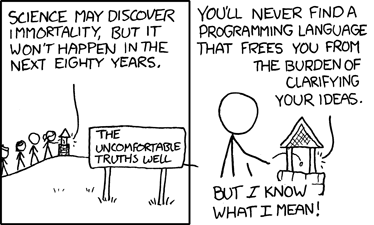
\includegraphics{./media/comics/well_2.png}
\end{quote}
From the \texttt{xkcd} comic “\href{https://xkcd.com/568/}{Well 2}” 

\subsubsection{Example of a process}
\label{sec:orgcaf9edf}

Consider the mathematical function \(f(x) = x + 10\).
\begin{itemize}
\item On its own, this function is not a process;
\begin{itemize}
\item it is only a \emph{rule} that \(f(x)\) is related to \(x + 10\).
\end{itemize}
\end{itemize}

However, you likely learned as a child
a “program” describing the process for calculating \(f(x)\).
\begin{minted}[breaklines=true]{text}
start with all your fingers down
say “x” 
repeat until you run out of fingers:
  say the result of adding one to the number you just said
  put up one finger
the answer is the last number you said
\end{minted}

In computing, we sometimes conflate programs and (mathematical) functions.
\begin{itemize}
\item Sometimes, we must remember they are not the same.
\item Mathematical functions are rules. They do no computing.
\item Programs describe a sequences of steps.
They may tell us how to compute
the results of mathematical functions.
\end{itemize}

\subsection{What are the components of a programming language?}
\label{sec:orgc8d6318}

Just like a natural language, a programming language consists of
\begin{itemize}
\item \emph{syntactic} rules
\begin{itemize}
\item which describe the legal forms of programs, and
\end{itemize}
\item \emph{semantics} rules
\begin{itemize}
\item which describe the meaning of legal programs,
\begin{itemize}
\item if they in fact have a meaning!
\end{itemize}
\end{itemize}
\end{itemize}

\subsubsection{Syntax and semantics example}
\label{sec:orge1e9532}

For example, English syntax tells us a sentence structured
\begin{minted}[breaklines=true]{text}
adjective adjective (plural noun) (plural verb) adverb
\end{minted}
is grammatically correct.

In the same way, a Python compiler tells us a program of the form
\begin{minted}[breaklines=true]{python}
expression + expression
\end{minted}
is syntactically correct.

Note that in both cases, though, such sentences/programs
may be meaningless!
Noam Chomsky gave the example
\begin{quote}
Colourless green ideas sleep furiously.
\end{quote}

And we could construct the Python program
\begin{minted}[breaklines=true]{python}
1 + "hello"
\end{minted}
which crashes when run.

\subsubsection{Exercise: a meaningless C or Java program}
\label{sec:org0adb9e7}

Our example Python program above
\begin{minted}[breaklines=true]{python}
1 + "hello"
\end{minted}
is syntactically correct because Python is \emph{dynamically typed},
meaning that type errors such as this are not caught until runtime.

As an exercise, can you construct a similar example
of a program which is syntactically correct
but semantically meaningless in the \emph{statically typed} languages
C and Java?

Hint: consider using a value which does not have just one type.

\subsection{How do we classify a programming language?}
\label{sec:orge8c69ff}

First and foremost, we classify languages into \emph{paradigms},
\begin{itemize}
\item characterised by the set of \emph{abstractions} the language makes available.
\end{itemize}

But also in many other ways, such as:
\begin{itemize}
\item Typing properties, including
\begin{itemize}
\item static or dynamic (runtime) typechecking,
\item “weak” or “strong” typing discipline,
\item polymorphism support, builtin types, methods of defining new types, etc.
\end{itemize}
\item “High” or “low” level languages.
\item (Primary) implementation strategy: compiled or interpreted?
\item Ancestery or culture.
\begin{itemize}
\item “Scripting languages”
\item “JVM languages”
\item “The C-family”
\begin{itemize}
\item \url{https://en.wikipedia.org/wiki/List\_of\_C-family\_programming\_languages}
\end{itemize}
\end{itemize}
\end{itemize}

\section{Abstraction}
\label{sec:orgdec9f17}
In “Concepts, Techniques and Models of Computer Programming”,
Peter Van Roy and Seif Haridi offer this definition of abstraction.
\begin{quote}
We define an
abstraction loosely as a tool or device that solves a particular problem. Usually the
same abstraction can be used to solve many different problems. This versatility
is one of the key properties of abstractions.
\end{quote}

In “Concepts of Programming Languages” (10th edition), Robert W. Sebesta
defines it so.
\begin{quote}
Briefly, abstraction means the ability to define and then use
complicated structures or operations in ways
that allow many of the details to be ignored.
\end{quote}

\subsection{Dijkstra on abstraction}
\label{sec:org5700042}

\begin{itemize}
\item A key feature of abstractions is that they let us set aside details
and work at a \emph{higher level}.
\item It is a common misconception that abstractions simply ignore details,
and in doing so lose precision.
\begin{itemize}
\item This thinking makes abstraction seem harmful.
\end{itemize}
\item Instead, abstraction involves selecting
\begin{itemize}
\item which details are relevant to the problem at hand, and
\item which details are irrelevant to the problem at hand.
\end{itemize}
\item When we set aside details that are irrelevant to a problem,
we can create solutions which will work for other problems
which share the same important details.
\end{itemize}

In his ACM Turing Lecture, “The Humble Programmer” in 1972, Dijkstra said
\begin{quote}
The purpose of abstraction is not to be vague, but to create
a new semantic level in which one can be absolutely precise.
\end{quote}

\subsection{Example: sorting}
\label{sec:orgdbf00c9}

Consider a programer who is assigned the following tasks.
\begin{enumerate}
\item Design a program which sorts a list of
dollar amounts in increasing order.
\item Design a program which sorts a list of
bank accounts in increasing order of the amount in the account.
\item Design a program which sorts a list of
bank customers in increasing order of the sum of the amounts
across all of their accounts.
\end{enumerate}

This programmer may write three programs which all look very similar,
except for
\begin{itemize}
\item the type of the input and
\item the method of access the values compared during sorting.
\end{itemize}

Or the programmer may realise that if abstract away these details,
so the program is made
\begin{itemize}
\item to accept any type (is made polymorphic) and
\item to take as an additional input the method of comparison,
\end{itemize}
the same code may be reused for all three tasks!

\subsection{“Leaky” abstractions}
\label{sec:org88cacb3}


When we use an abstraction, we intend to hide unimportant details.
But in some cases, those details may still be exposed.
\begin{itemize}
\item We say they “leak through”, so we have a “leaky abstraction”.
\end{itemize}

A classic example is iterating over a two-dimensional array.
\begin{itemize}
\item Two-dimensional arrays allow us to reason about a square made of memory cells.
\begin{itemize}
\item In a two-dimensional array \texttt{A}, it would seem \texttt{A[1][1]} is adjacent
to \texttt{A[0][1]}, \texttt{A[2][1]}, \texttt{A[1][2]}, and \texttt{A[1][0]}.
\end{itemize}
\item But computer memory is one-dimensional.
\begin{itemize}
\item A cell of memory cannot be adjacent to four others; only two.
\end{itemize}
\item Iterating through two-dimensional arrays in the wrong direction
can be very inefficient when the array is large.
\begin{itemize}
\item If \texttt{A[1][1]} and \texttt{A[2][1]} are in fact not adjacent,
and are in separate caches or on separate pages,
we will trigger a cache miss or page fault
by iterating through in the second dimension.
\end{itemize}
\end{itemize}

\subsection{A taxonomy of programming paradigms by abstraction support}
\label{sec:org2fd130b}

From Peter Van Roy's 2012 paper,
“\href{https://www.info.ucl.ac.be/\~pvr/VanRoyChapter.pdf}{Programming Paradigms for Dummies: What Every Programmer Should Know}”.

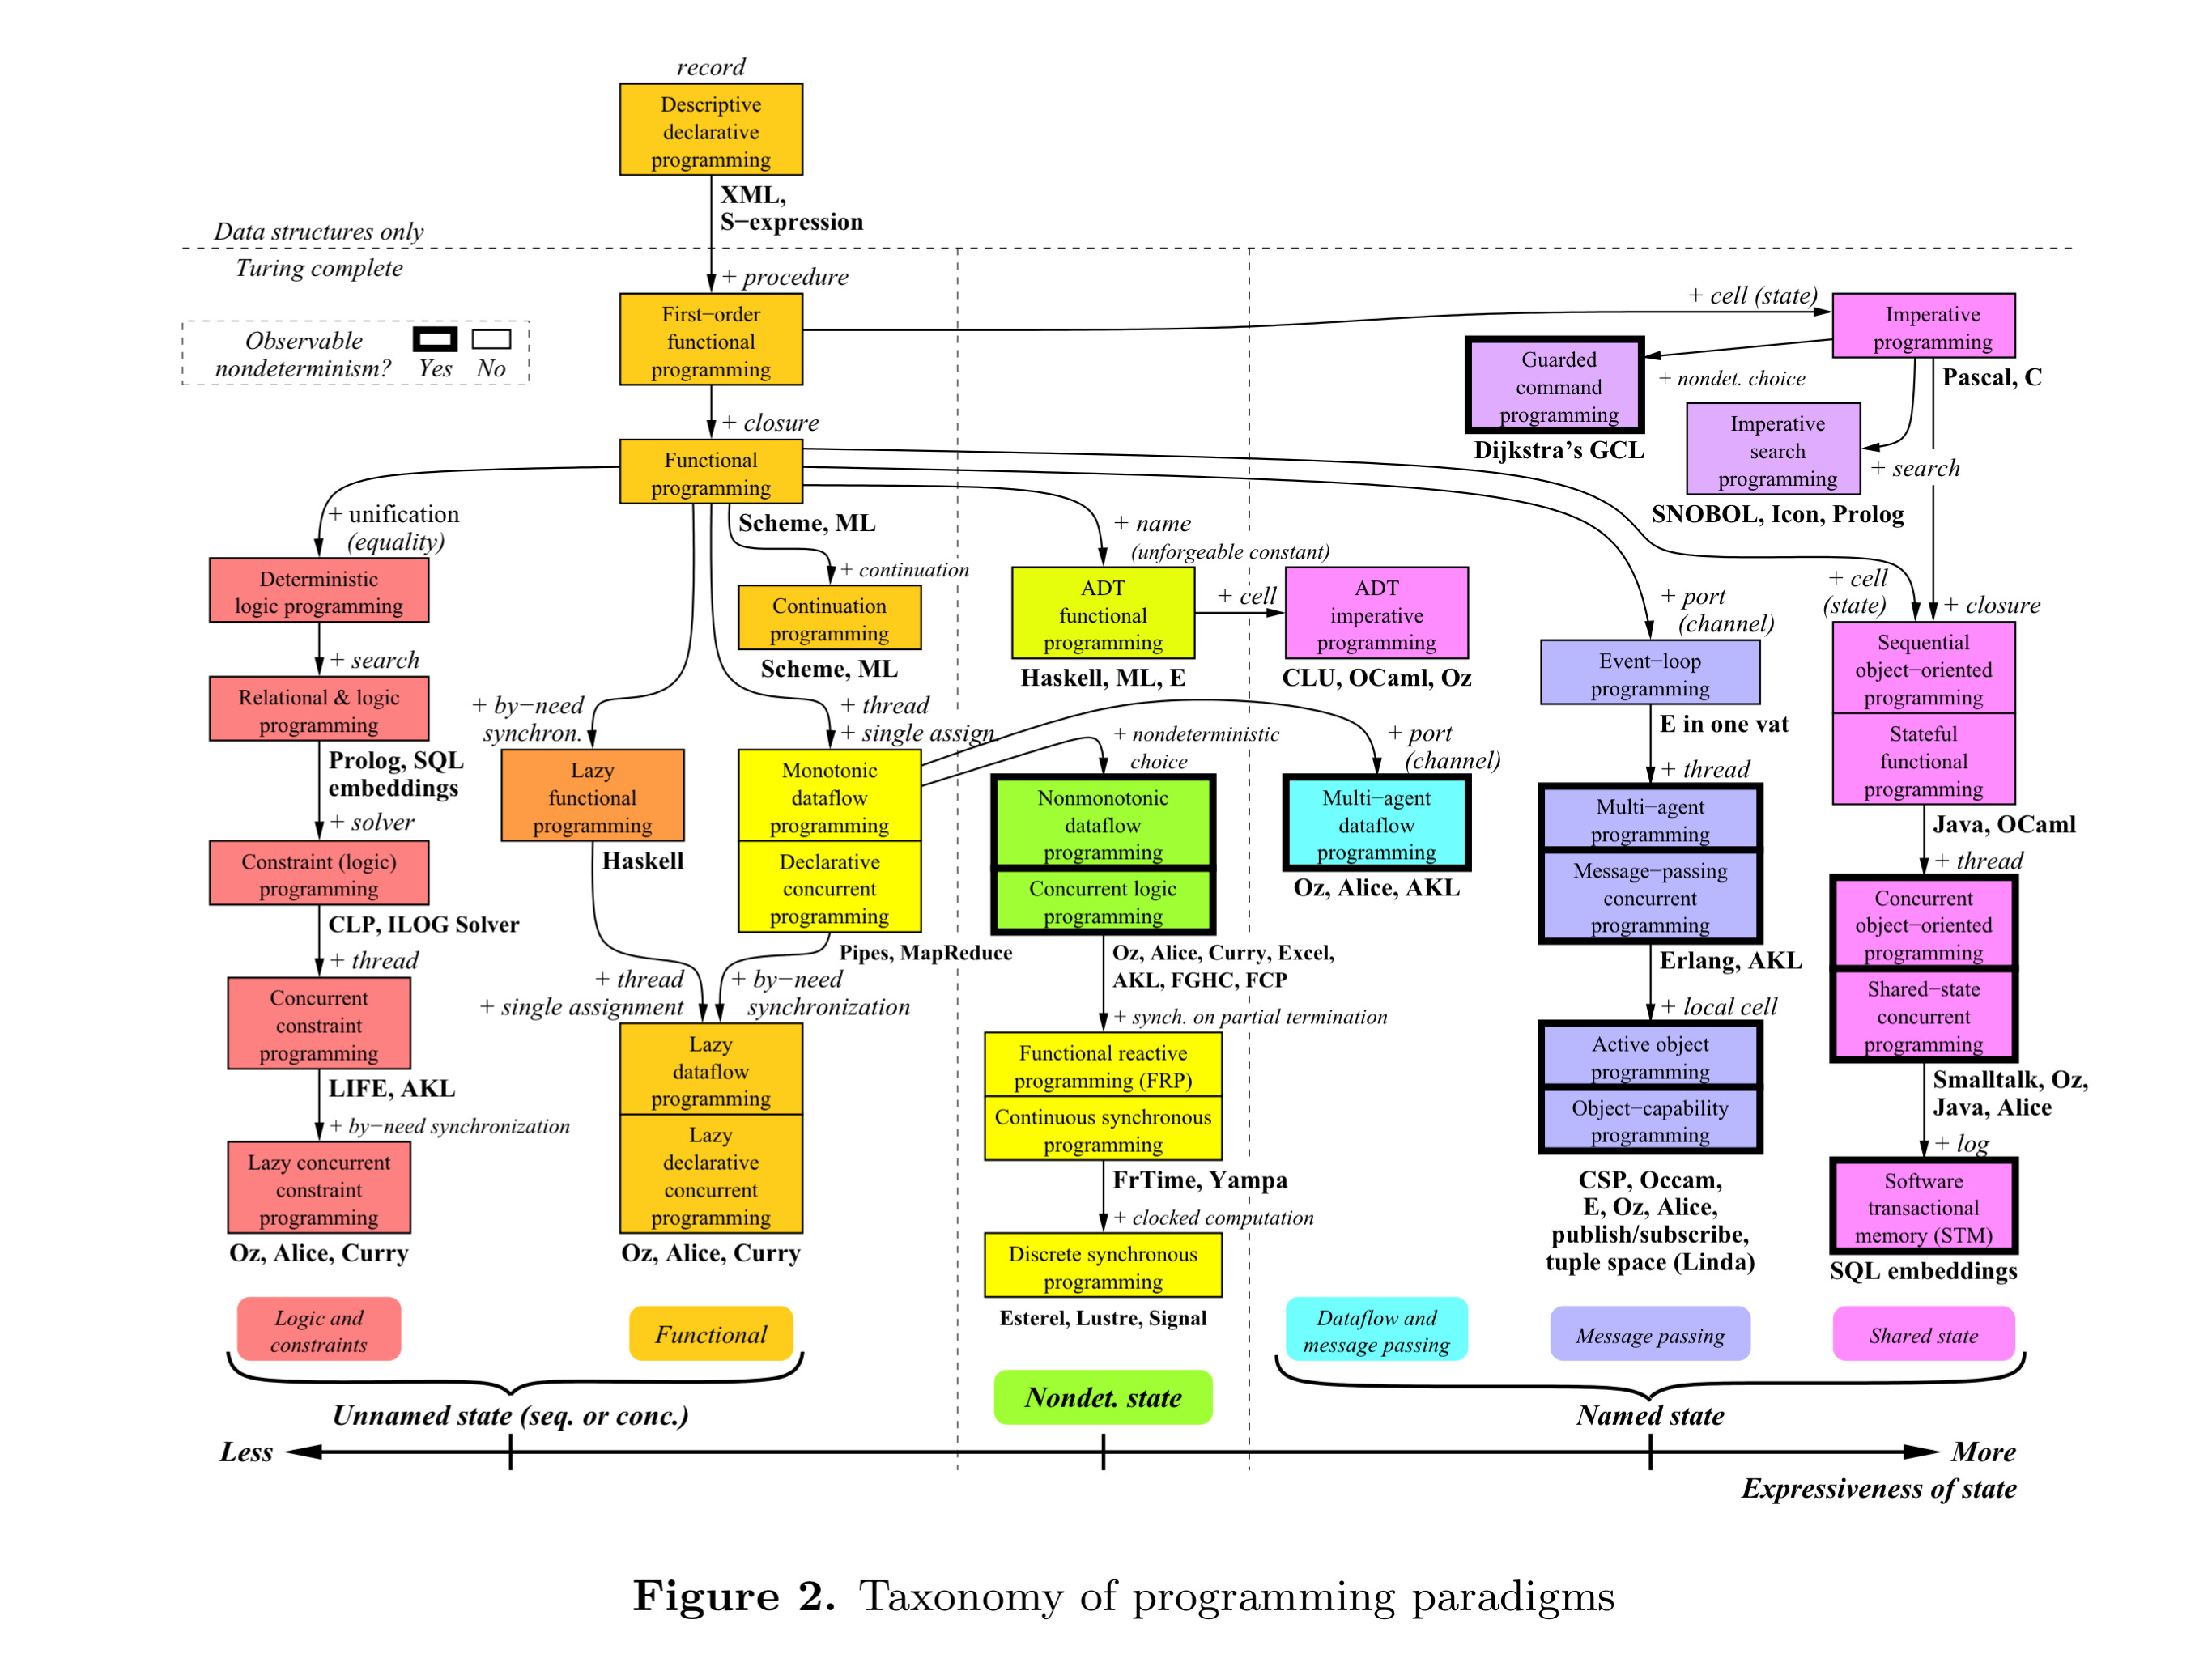
\includegraphics[width=\textwidth]{./media/vanroy-paradigm-chart.png}

\subsection{Abstractions throughout this course}
\label{sec:org5445a47}

We will see numerous abstractions throughout this course.
\begin{itemize}
\item Functions, methods, procedures and subroutines abstract away from
managing control flow.
\item Variables abstract away from reasoning about the contents of
registers and memory.
\item Abstract data types abstract away from the form of data in memory.
\item Reference types abstract away from reasoning about memory addresses.
\end{itemize}

We will also try to de-mystify some abstractions
which are often considered difficult to understand.
\begin{itemize}
\item Algebras abstract away from sets together with operations on those sets.
\item Closures abstract away from the concept of a function
existing alongside some state.
\item Monads abstract away from choosing a particular computation strategy.
\end{itemize}

\section{Exercises}
\label{sec:org6e1a57f}
\hyperref[sec:org0adb9e7]{Exercise: a meaningless C or Java program}
\end{document}
